\chapter{Dataanalyse}
I denne fasen analyseres vi dataene som er samlet inn, vi har ganske lite data i dette caset, derfor har vi ganske få valgmuligheter for bruk av verktøy i følge boken \cite{RCA}. Dataene er heller ikke på nummerisk form, som flere av analyseverktøyene krever.

\section{Affinitetsdiagram}
Affinitetsdiagram brukes til å analysere data som det ikke er mulig å nummerere, eksempelvis meninger eller ideer. Affinitetsdiagram grupperer data og finner de underliggende korrelasjoner og likhetstrekk i gruppen.


\section{Ønsket utbytte}
Ønsket utbytte av å bruke affinitetsdiagram er å finne bindinger eller fellesnevnere som kan være til hjelp for å fjerne rotårsaken. 

\section{Gjennomføring}
Analysen ble gjennomført med å ta transkripsjon av intervjuet og stykke den opp i fem hovedgrupper.     

\section{Resultat}

\begin{figure}[H]
    \centering
    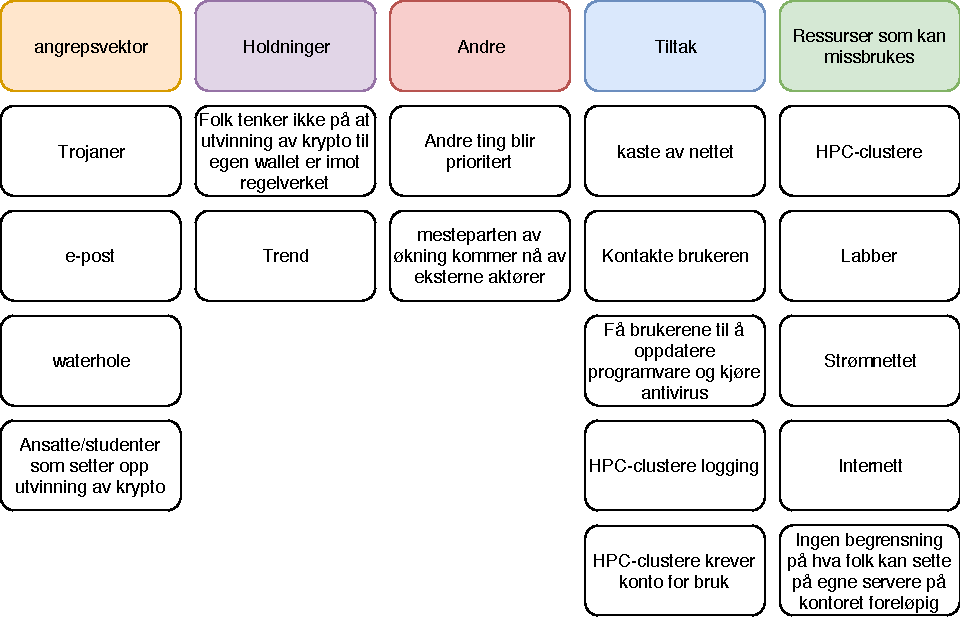
\includegraphics[scale=0.6]{case_3/bilder/AD.pdf}
    \label{fig:AD_miner}
    \caption[Analyse av intervju]{Hvordan fungerer utvinning av kryptovaluta ved NTNU?}
\end{figure}

Vi finner mulige årsaker og tiltak som er satt på plass, og forhåpentligvis er rotårsaken blant dem.

\section{Konklusjon av verktøy}
Verktøyet fungerte godt, selv med en liten datamengde. Vektøyet er effektivt til å strukturere transkripsjonen fra intervjuet til mer brukbare og oversiktlige nøkkelpunkter. 
